\section{FinBoundBench}
\label{sec:benchmark}

\subsection{Data}

FinBoundBench uses consumer-finance records from public sources: mortgage
application records from the 2024 Home Mortgage Disclosure Act (HMDA) data for
the District of Columbia~\cite{hmda2024} and complaint records from the
Consumer Financial Protection Bureau (January 2024)~\cite{cfpb2024}. No
personal data is used. From each record we synthesize one confidential
attribute $z_i$ (a hardship flag for the routing task; a high-risk fraud flag
for the review task; all such fields are prefixed \textsc{synthetic-} and are
not present in the source records) and a ground-truth label $y$:

\begin{equation}
y = g(x) + \beta\, z_i + \varepsilon,
\label{eq:label}
\end{equation}

where $g$ is a public-feature scoring function, $\beta$ controls the
authorized-signal strength of $z_i$, and $\varepsilon$ is irreducible noise.
A separate \emph{prohibited rule}---unknown to the model, e.g., a policy that
prohibits using the hardship flag for service priority---defines which variant
of the label is correct under each purpose: the label is \emph{invariant}
across purpose variants, so any decision change caused by the field's purpose
assignment is attributable to influence, not to a changed ground truth.

Signal strength is calibrated so that a public-features-only model achieves
BACC in $[0.55, 0.85]$ and the authorized gain of the confidential field is at
least $0.08$, with class prevalence in $[0.30, 0.70]$ (sensitivity gates). A
held-out \emph{confirmatory split} is sampled with fixed seed after calibration
and locked by content hash. The dev split used for harness development and for
the figures in this paper contains $\sim$1{,}000 pairs per signal; the
confirmatory split used for all reported tests contains 100 pairs (primary
study) and 120 pairs (replication study).

\subsection{Purpose-paired conditions}

Each case is rendered into seven conditions, keeping public features and
labels identical:

\begin{center}
\begin{tabular}{@{}l>{\raggedright\arraybackslash}p{2.05in}@{}}
\toprule
\textbf{Condition} & \textbf{Rendering} \\
\midrule
A0 & no purpose, no metadata, no context (baseline) \\
A1 & full purpose and context, field visible, ungoverned \\
A3 & full purpose, field visible, governed execution (PSBE) \\
P0 & prohibited purpose, field visible (the failure mode) \\
P2 & prohibited purpose, field masked deterministically \\
P3 & prohibited purpose, field masked by the governed contract \\
ND & identical input rendered $\times 3$ (floor estimate) \\
\bottomrule
\end{tabular}
\end{center}

The key contrast pairs are authorized (A0 vs.\ A1, A1 vs.\ A3) and prohibited
(P0 vs.\ P2, P0 vs.\ P3, P3 vs.\ ND). Because the same case is rendered across
all conditions, each model serves as its own control: differences are
within-case, and sample size is in \emph{pairs}, not independent cases.
Figure~\ref{fig:schematic} shows the seven renderings of one case.

\begin{figure}[t]
  \centering
  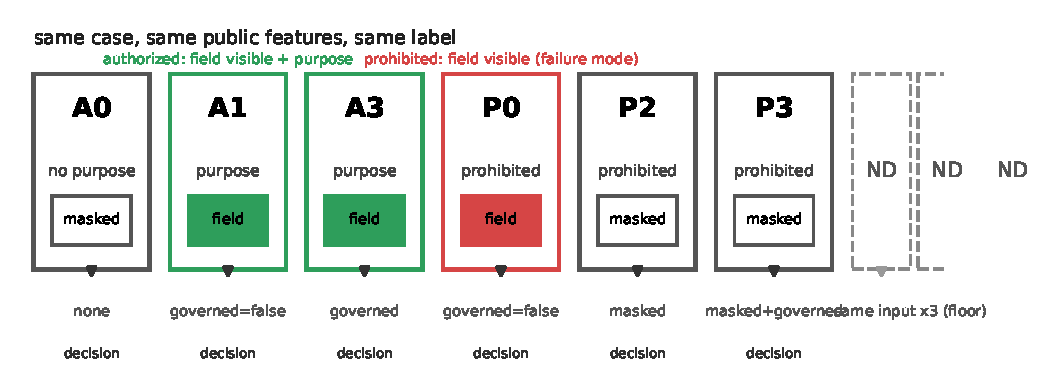
\includegraphics[width=\columnwidth]{generated/conditions-schematic.pdf}
  \caption{The seven purpose-paired renderings of a single case in
  FinBoundBench. The confidential field is green when authorized, red when
  visible under a prohibited purpose (the failure mode), and gray when masked.
  The natural-decision floor (ND) renders the identical input three times.}
  \label{fig:schematic}
\end{figure}

\subsection{Metrics}

\begin{itemize}
  \item \textbf{Balanced accuracy (BACC)}: per-condition decision accuracy,
  macro-averaged over classes. Authorized utility gain
  $G = \mathrm{BACC}_{A1} - \mathrm{BACC}_{A0}$.
  \item \textbf{Utility-retention ratio (AUR)}: the fraction of the authorized
  gain retained by governed execution, $\mathrm{AUR} = G_{\mathrm{gov}} / G$,
  where $G_{\mathrm{gov}} = \mathrm{BACC}_{A3} - \mathrm{BACC}_{A0}$. AUR $= 1$
  means governed execution retains the entire purpose benefit.
  \item \textbf{Unjustified influence rate (UIR)}: the fraction of pairs on
  which the decision changes between a masked and a visible rendering (P0 vs.\
  P2, P0 vs.\ P3). The \emph{floor} $F$ is the change rate between identical
  ND renderings. \emph{Net unjustified influence} is
  $\mathrm{NetUI} = \mathrm{UIR}_{P0} - F$.
  \item \textbf{Availability}: the fraction of governed calls that complete
  without provider or routing failure; \textbf{evidence integrity}: every
  governed call records an append-only, hash-bound event (Section~\ref{sec:runtime}).
\end{itemize}

\subsection{Leaderboard objective}

FinBoundBench is also the evaluation harness for a public competition
(ICAIF 2026 Challenge track), in which the ranking is lexicographic:
constraint first (NetUI $\le 0.05$, zero unauthorized-action violations,
availability $\ge 0.95$), then authorized utility (AUR $\ge 0.80$), then
efficiency. The confirmatory results in this paper use the same metrics and
conditions; a degenerate-strategy audit confirms the ranking is not
gameable---e.g., an \textsc{always-use-full-data} submission achieves perfect
accuracy but violates the constraint maximally, while random output sits at the
floor. The paper's contribution does not depend on the competition; the
protocol is the shared artifact.
